draft

	
\chapter{Le Journal Officiel : la parole, la main, la vue et le droit}
%\input{exemple_section1.tex} %Input: importer un fichier
\epigraph{\itshape Dorénavant, la promulgation des lois et des décrets résultera de leur insertion au Journal officiel de la République
	française, lequel, à cet égard, remplacera le Bulletin des lois.}{Décret 1870-11-05 Bull. des lois, 12 S., B. 29, n° 169}


Le \textit{Journal Officiel} constitue la matière documentaire pour notre cas d'usage, lequel porte sur la qualité des débats parlementaire dans les années trente. Ce n'est pas qu'une matière qui témoigne et publicise l'activité politique institutionnelle : elle fait passer, depuis au moins la Révolution Française, les paroles des délibérations dans le droit effectif. Et entre la parole et la lettre, le travail des sténographes et rédacteurs qui établissent des transcriptions. 

Ces documents sériels publiés quasimment quotidiennement depuis la Révolution Française, établissent les débats politiques et les décrets qui entérinent les lois. Selon Hugo Coniez, ces sources sont étrangement une matière assez peu exploitées même si elles seraient fort utiles à l'élaboration d'une histoire politique des institutions françaises. Du point de vue de l'ingénieur documentaire ou de l'historien-ingénieur, la monotonie et le gigantisme de ces sources est une aubaine car il semble que l'on pourrait extraire de façon industrielle de l'information. Ces documents, avec une composition typographique relativement sobre, seraient des \enquote{fruits faciles}, prêts à cueillir. 

Ce chapitre consacrera une analyse formelle et une mise en contexte historique de ces sources qui est à faire commencer à la Révolution Française. Il me faut mentionner d'emblée le travail de Fanny Lebreton -- stagiaire pour le projet AGODA, génétique au projet Mezanno -- qui établit déjà une synthèse sur le sujet, en particulier à l'endroit du travail sténographique. Dans son mémoire, elle a rédigé une synthèse de l'histoire des publications officielles. Je risque de me répéter; si bien que j'essairai d'aborder cette histoire avec des éléments complémentaires, en rappellement bien évidemment les jalons les plus important pour donner indépendance à mon propos. Pour compléter cette histoire à titre de contextualisaiton des sources, il s'agira de mettre en perspective l'histoire des \textit{journaux officiels} avec celle des stratégies de \textit{promulgation} des lois dont l'exercice exécutoire repose sur des stratégies documentaires, lesquelles incluent également l'affichage administratif. Ceci, on le verra, permettra de comprendre notamment la présence de journaux édités -- qui ne sont donc pas à proprement parler des archives -- dans les services d'archives départementaux. Cela me conduit à prendre le point de vue non pas des différentes publications et de ce qu'elles récupèrent en héritage ; mais de celui de l'activité parlementaire et de la problématique de la promulgation des lois et de leur publicité. Voilà comment cette activité se donne en partage : les délibérations au seins des institutions (pratique orale); la rédaction de comptes-rendus de ces délibérations (pratique écrite); leur publicité  (donner à la connaissance des administrés la loi); et l'effectivité du droit, qui passe par la publication de documents écrits.

Egalement, grâce aux archives de la Direction du Journal Officiel conservées aux AN, je tenterai d'apporter quelques éléments nouveaux en portant attention au travail administratif et technique de celles et ceux qui font le journal officiel -- rotativiste, lynotypiste, rédactrices, sténographes, secrétaires.

\begin{quote} (Cette attention construite pour fournir un contexte à mon propos ne pourra pas, cependant, se substituer à un travail de recherche historique qui se dédierait à cette question. Le chercheur interressé à la question pourra consulter la série 19840069/1-6 des Archives nationales).\end{quote}

Dans cette partie on donnera donc 1) la chronologie générale du Journal Officiel; 2) une clarification des typologies documentaires (archives, bibliothèque); 3) une analyse des "processus métiers" et ainsi des documents produits dans le cadre de l'activité de publicisation parlementaire. Il faudra regarder aussi bien du côté des Chambres dans les années 30 que du côté des "gratte-papiers" de l'administraiton du JORF. Et enfin 4) l'analyse des documents qui seront soumis aux traitements d'extraction d'entité nommées.

\noindent\makebox[\textwidth]{%
	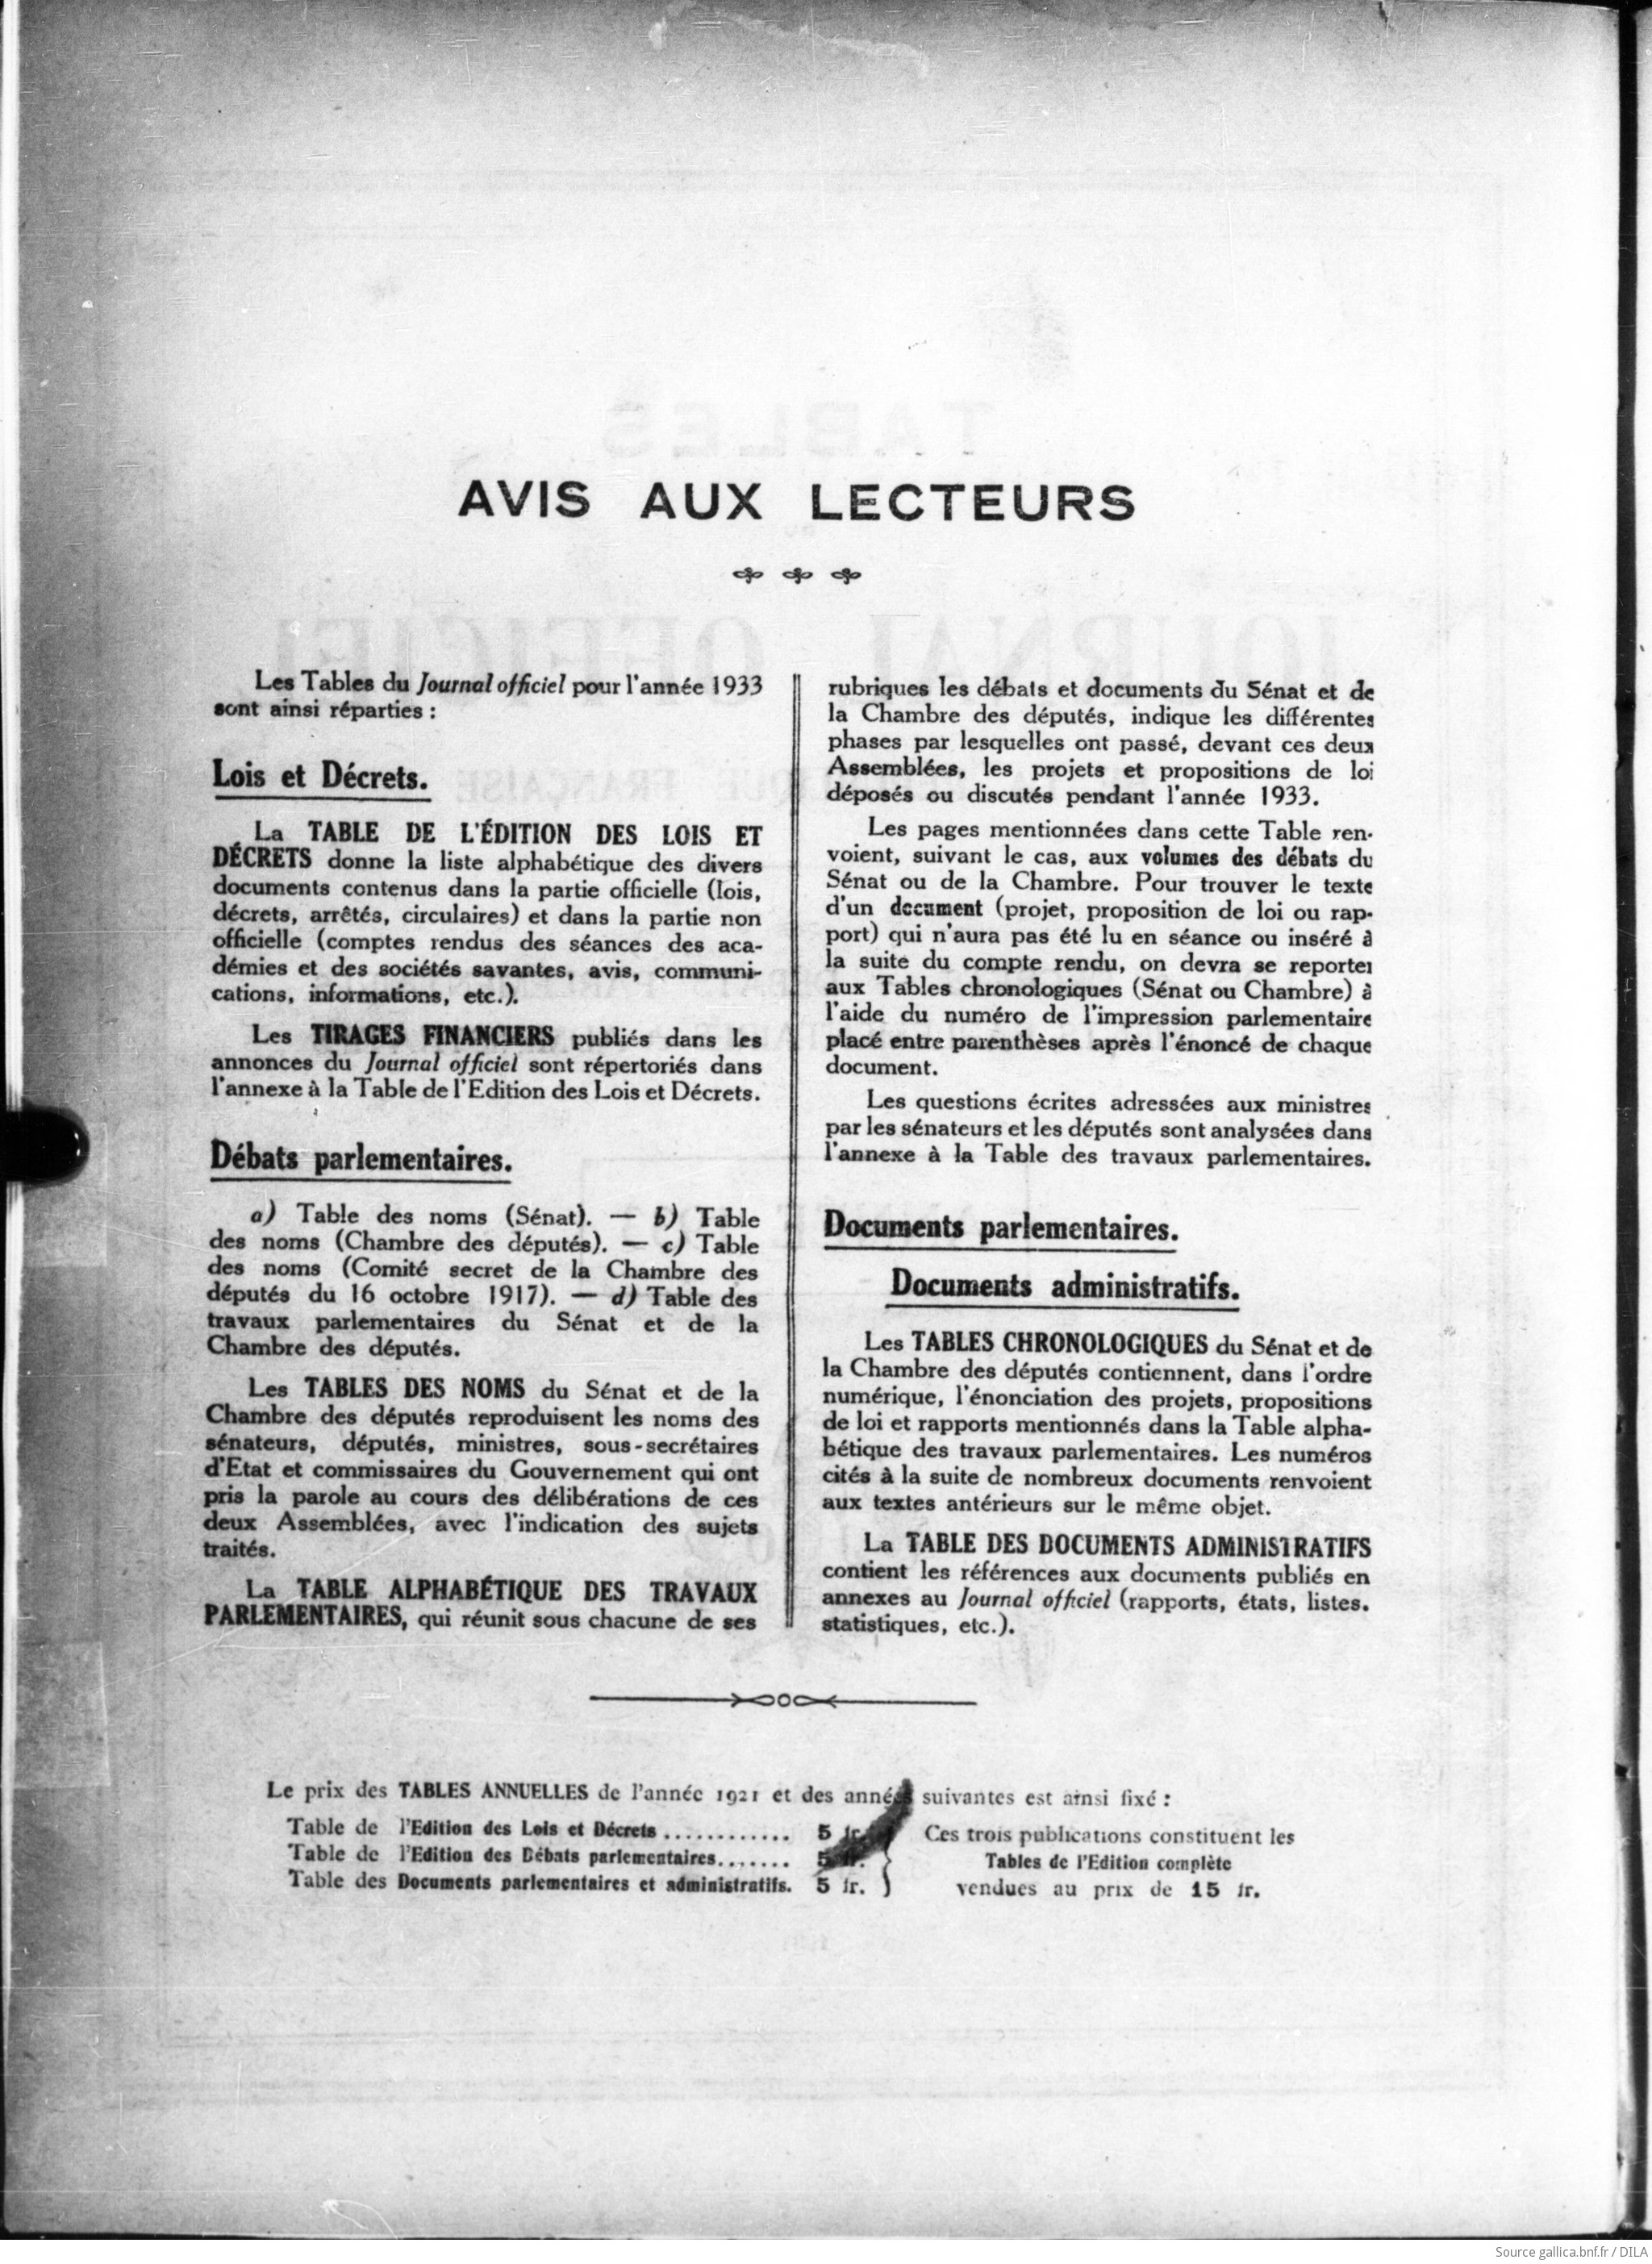
\includegraphics[width=\paperwidth,height=\paperheight,keepaspectratio]{test.jpeg}%
}

\section{Le Journal Officiel de la IIIe République : publiciser, publier, promulguer l'activité parlementaire}

Le {Journal Officiel} a une double fonction : la première, de teneur révolutionnaire, de faire la publicité de l'activité parlementaire à travers des comptes-rendu; la seconde d'entériner la valeur exécutoire d'une loi -- la promulguer -- par la publication. Ces fonctions du \textit{Journal Officiel} ne sont pas exclusives à la IIIe République, elles trouvent leur origine, comme le principe de transparence des institutions publiques, à la Révolution française.

\section{Délibérer, voter la loi}

\section{Publiciser l'activité parlementaire}

\section{Promulguer, publier}

On entend le son d'un cuivre, une foule se constitue autour du trompettiste accompagné du juré-crieur : une nouvelle loi est \textit{publiée}.

Promulguer = moment où la loi s'applique; mais ce qui entérine cette application, c'est la publication.


Deux branches chronologiques et une fusion : \textit{Le Moniteur Universel*, *Le bulletin des lois}, le JO.

Publication et notification. Deux modalités de publicité.

Révolution française : Moniteur 1789 - 1869 (puis JO sous adjudication); Bulletin des lois 1793 / 1931; puis le "merge" final en 1931 dans la branche "JO", qui existe depuis 1869.

Adjudication ; régie ; 1870 + la Commune ; 1914/18; 39/45 ; 45/2010 + (réforme de 76) aujourd'hui. Parler de la Société Anonyme ouvrière.

A noter évidemment la réorganisation des administrations de l'Etat sous le Régime de Vichy: en 1940...

\section{1921 -- 1940. Un aperçu du fonctionnement technique et administratif du Journal Officiel}

Faire une histoire à grain fin de la façon de fabriquer et lire le Journal Officiel de ses débuts à aujourd'hui serait une étude fort passionnante. En tout cas, même avec un bornage chronologique plus modeste, elle peut être utile à donner davantage de substance au contexte de la source qui sera traitée pour répondre à une question de recherche. Mais ce n'est pas ici mon objet : me voilà bien obligé de me restreindre aux dates qui concernent ma question de recherche (l'activité parlementaire entre 1931 et 1935), et de lui adjoindre quelques marges en guise de fondu chronologique. Je tombe à 1921 et 1940. Pourquoi ces dates ?

Parce que 1921 correspond à la date d'acquisition d'un nouveau matériel technique, la \textit{linotype Model 9}; et 1940 marque l'interruption des parutions du J.O. et la réquisition du matériel sous ordre de la Police Militaire Allemande (Source: 19840069). Le matériel joue sur la façon de produire le journal et il semble y avoir une certaine uniformité dans la façon de produire le journal pendant cette période. Je ne me soucirai donc pas de savoir si, en deça de ces bornes, la façon de produire le \textit{Journal} est fondamentalement différent, même si, on s'en doute, étend donné les délais de publication du J.O. qu'il soit possible de dégager une structure générales des méthodologies employées.

Personnels, budget.

Formalités techniques du JO (années 20/30) : la "Doric". lynotype 9 qui permet jusqu'à 4 "faces" en même temps.

- La "doric" (ou )

\section{Le Journal Officiel : des \enquote{archives} ?}

Le \textit{Journal Officiel* est une *publication* et dont la gestion incombait - et incombe toujours - à l'exécutif. La *Direction des Journaux Officiels*, depuis le décret du 30 décembre 1880 jusqu'à l'ordonnance du 2 novembre 1944, est placée sous la tutelle administrative du *Ministère de l'Intérieur}, à travers l'action d'un préfet nommé Directeur, à l'occasion d'un Conseil des Ministres. La nomination est actée par décret. A noter que ce Directeur, chargé la direction et de la surveillance des services, rédige un rapport à l'adresse du 1er Ministre sur les résultats de l'exploitation des J.O., qui n'est pas publié : c'est un document opérationnel sans valeur juridique mais qui peut se retrouver, par exemple, dans les archives de la Mission d'organisation des services du Premier Ministre.

\begin{quote} 19970278 AN\end{quote}

Comme on l'a vu, la direction comprend en fait seulement la partie admininistrative et commerciale. Les impressions du journal, elles, sont en fait gérées par la "Société anonyme à capital variable de composition et impression des Journaux officiel de la République Française" (SACIJO), placée en régie depuis 1880/1881. Malgré la création de la DILA en 2010 chargé, entre autres (c.f. missions de la Documentation fr) de la publication numériques des J.O., la SACIJO existe encore aujourd'hui et devrait exister, comme l'exige l'article 19 de ses statuts, jusqu'en 2050.

Plus encore, les textes présentés sont l'expression d'un travail d'interprétation à plusieurs mains : ils sont écrits, retouchés, rédigés en vu d'être lus. C'est donc un véritable travail éditorial. Parler "d'archives" serait donc ici un abus de langage, si l'on considère la définition juridique française, à savoir les archives comme le produit organique d'une activité donnée, distincte des oeuvres de l'esprit ou de ce qui est couvert par le Dépôt légal (art. 211-1 du Code du Patrimoine).

En effet, le \textit{Journal Officiel* -- je ne m'intéressai qu'à la version papier donc de 1869/2010 -- est imprimé et *vendu* : il est donc soumis au *Dépôt Légal} et est à ce titre conservé à la BnF. Il est bien sûr consultable au Sénat et à l'Assemblée nationale pour des raisons opérationnelles et patrimoniales; ainsi qu'à la bibliothèque des Archives nationales. Si les Archives nationales considèrent bel et bien les JO comme de la documentation -- étant rangées à la bibliothèque et donc en-dehors d'un cadre de classement archivistique --, le cas est différent pour les Archives départementales. En effet, chaque Département conserve, au sein de la série K institué par l'ordonnance du 24 avril 1841 qui réforme les cadres de classement des AD ayant pour mission de centraliser les archives de la Nation à l'échelon départemental, les publications officielles de l'Etat.

De façon naïve, en vertu de la séparation des pouvoirs, cette gestion côté executive de l'édition de l'activité parlementaire peut paraître dissonante. Pour commencer, il


\section{Les \enquote{processus métier} de l'activité parlementaire de la IIIe République}

\enquote{Processus métier} : un terme anachronique pour dire que l'on veut cartographier l'exercice parlementaire -- et donc avoir une idée des archives qui sont produites dans le cadre de cette activité. Un terme anachronique pour dire aussi qu'il n'est pas question de faire une histoire politique de la Troisième République. C'est ici une approche archivistique qui est envisagée car l'enjeu ici est de travailler sur le liage d'informations, issues de sources diverses -- et donc de qualifier les sources. Cette approche permetttra, je l'espère, de comprendre comment "mûrissent les dossiers" sur l'établi du parlementaire -- et donc de voir de quels arbres sont les articles publiés dans le \textit{Journal Officiel}.

S'intéresser à la façon dont murissent les dossiers. Partir du point de vue du papier remuer, donc de l'activité administrative qui produit des documents (archives). Ajdh L'accès à ces archives dépendent des réglements des deux chambres. Mais la publicité de l'activité parlementaire, bien entendu, est garantie par un travail \textit{éditorial} -- ce qui pourrait poser la question du droit d'auteur des sténographes ! -- et l'expression de ce travail est le JO. J'aborde le problème du général au particulier, du cadre théorique posé par la constitution à l'organisation du travail parlementaire au niveau des bureaux.

\subsection{Du point de vue constitutionnel}

Avant cela, il convient de fournir le cadre juridique global qui, en théorie, encadre les pratiques parlementaires. Ce cadre est donné par la Constitution de 1875, fruit de trois lois (deux en février, une en juillet) et des révisions (XXXX, XXXX).

La IIIe République est composée d'un exécutif bicéphal (le président de la république et le Chef du gouvernement, c'est à dire le président du Conseil des Ministres, rôle équivalent aujourd'hui du Premier Ministre; mais ce qui ne veut pas dire qu'il jouent un rôle équivalent) avec un fonctionnement législatif bicaméral. Attention, car la Constitution de 1875 appelle "Assemblée Nationale" l'addition de la Chambre des Députés et du Sénat.

La Constitution, qui établit le fonctionnement général de l'organisaiton des pouvoirs publics et de ses institutions, a été modifiée plusieurs fois. On rappelle également le principe de séparation des pouvoirs : le législatif peut délibérer des lois et les faire voter" -- processus parlementaire, l'exécutif les appliquer (par décret, arrêtés ou ordonnances). La pyramide des normes, en plaçant le levier d'action de l'exécutif au niveau du bloc réglementaire en-dessous du bloc de légalité, rend (en pratique) possibile la logique de contrôle des parlementaires sur le gouvernement et le président. Un président de la IIIe République peut cependant proposer des lois, mais qui doivent impérativement passer par les chambres.

Cependant, l'organisation du travail des lois n'est définie dans la Consitution que de façon macroscopique (elle expose le fonctionnement institutionnel général ainsi que les sessions) : Le pouvoir législatif s'exerce par deux assemblées (chambre des députs + sénat). Le président et le pouvoir législatif peuvent faire voter ou voter les lois; le président peut les promulger. Sans entrer dans le détail de l'élection, il faut noter que c'est l'Assemblée nationale -- donc le Sénat et la Chambre -- qui élit le Président. Le sénat est élu par ...

On remarque également, à la lecture des lois constitutionnelles de 1875, que le Sénat est davantage consacré que la Chambre des Députés. La chambre basse, élu au suffrage universel, a moins de pouvoirs que le Sénat, qui peut autoriser la dissolution voulu par le président de la Chambre des députés. Le Sénat, lui, ne peut être dissous. Le Sénat a également la capacitéi de se constituer en cour de justice pour juger les têtes exécutives.

Les prérogatives :

- Chambres réunies en sessions de 5 moins minimum ("sessions parlementaires")

- le vote des lois, chaque chambre peut-être à l'initiative des lois

- le président doit déposer ses projets de lois dans n'importe quel "bureau" de n'importe quel chambre, qui les discute et les renvoie à l'autre

- La navette parlementaire: Si aucun accord n'est trouvé entre les deux chambres, la loi n'est pas votée (pas de préeminence d'une chambre sur l'autre)


En revanche, c'est un réglement, exclusif à chaque assemblée qui fait la description plus précise de l'organisaiton du travail parlementaire. Les réglements relatifs aux assemblées législatives s'appuient sur ceux de la IIe République -- il a fallu d'ailleurs s'organiser de façon similaire à la Seconde pour faire le réglement. Ils peuvent être connus grâce aux comtes rendu \textit{in extenso} des séances du Journal Officiel.

\begin{quote} La recherche s'est effectuée à partir du livre de Roger Bonnard !\end{quote}

\subsection{Le Sénat}

Ce sont par les séances du 7, 8, 9 et 10 juin 1876, rapportées respectivement dans les compte-rendus \textit{in extenso} du J.O. des éditions du 8, 9, 10 et 11 juin 1876, que l'on établit le réglement du Sénat, et donc l'organisation concrète de leur travail parlementaire.

- article 4 : le bureau définitif élu pour un an

- article 7 bureau définitif ==> sénat constitué

- article 11 "le sénat se partage en neuf bureaux, renouvelés chaque mois, en séance publique, par la voie du sort" "chaque bureau nomme son président"

- art 12 les bureaux se conforment [...] aux ordres du jour arrêtés par le Sénat. Chacun d'eux discute séparement les questions renvoyées à leur examen. 
Il est tenu procès verbal de leurs délibérations [et qui] mentionne les noms des membres présents

- art 13, délaisdiscussions

- art 14, chaque bureau, lorsque la discussion est terminée, nomme un commissaire (par vote, voir article 6)

- article 17 : sont nommées chaque mois par les bureaux :

- une commission chargée d'examiner les propositions émanement de l'initiative parlementaire et donner son avis

- une commission chargée de l'examen de projets de lois relatifs à des intérêts communaux et départementaux

- une commission chargée de l'examen des pétitions

- congés

- ces commissions sont composées de neuf membres (sauf la commission de l'initiative parlementaire qui en a 18)

- article 18 : Le Sénat [le bureau définitif ?] peut renvoyée à une commission déjà formée


\begin{quote} Réglement en annexe ? vérifier dates\end{quote}

\subsection{La Chambre des Députés}
Ce sont par les séances du 9, 10, 13 et 16 juin 1876, rapportées respectivement dans les compte-rendus \textit{in extenso} du J.O. des éditions du 10, 11, 14 et 17 juin 1876 que l'on tétablit le réglement du Sénat, et donc de l'organisation concrète de leur travail parlementaire. Mais c'est une réglementation très changeante, car théâtre de luttes entre différentes sensibilités idéologiques. Le \enquote{conservatisme} du Sénat rend possible un cadre qui évolue moins avec le temps. Peu de choses sur le système des commissions permanentes.

\begin{quote} Réglement en annexe ? Vérifier dates\end{quote}
%etc
%Ou bien: ne pas mettre chapter, et importer le chapitre complet:
%\input{mon_chapitre_1.tex}
%\input{mon_chapitre_2.tex}	
%etc

\chapter{Les tables annuelles : des relations entre corpus}
a
\section{Les tables dans l'environnement du \textit{J.O.}}
q
\section{Forme des tables}
q
\section{Informations sémantiques des tables}
s
\section{Les tables comme \enquote{hub} intercorpus}
s

\chapter{La qualité du débat démocratique de la IIIe République. Lire à distance}
Matériel quantitatif, lapidaire autant que monumental : envisager le \enquote{distant-reading}
\section{Distant reading ?}
\section{Outils statistiques généraux}
Abstraction des besoins par rapport aux données disponibles. Modélisation.



\part{Le projet Mezanno : aspects institutionnels et techniques}
OCR, Annotation NER. Etat de l'art.

application côté mezanno, avantage

Extraire les données

Génération structurée 
%etc.

\part{Appliquer l'outil Mezanno : étude de la qualité des débats parlementaires 1931--1935}

indicateurs

\chapter*{Conclusion}
fonds dormants ? valorisation
\addcontentsline{toc}{chapter}{Conclusion}
\newpage{\pagestyle{empty}\cleardoublepage}




